\documentclass[12pt]{article}%
%%%%%%%%%%%%%%%%%%%%%%%%%%%%%%%%%%%%%%%%%%%%%%%%%%%%%%%%%%%%%%%%%   
% All style files are available from 
%   http://wwww.uiuc.edu/~sariel/research/latex/
%%%%%%%%%%%%%%%%%%%%%%%%%%%%%%%%%%%%%%%%%%%%%%%%%%%%%%%%%%%%%%%%%%   


%%%%%%%%%%%%%%%%%%%%%%%%%%%%%%%%%%%%%%%%%%%%%%%%%%%%%%%%%%%%%%%%%%   
% Conditional compilation depending on whether this is my computer or
% not.
\IfFileExists{sariel_computer.sty}{\def\sarielComp{1}}{}
\ifx\sarielComp\undefined%
\newcommand{\SarielComp}[1]{}
\newcommand{\NotSarielComp}[1]{#1}%
\else
\newcommand{\SarielComp}[1]{#1}%
\newcommand{\NotSarielComp}[1]{}%
\fi
\newcommand{\IfPrinterVer}[2]{#2}%

%%%%%%%%%%%%%%%%%%%%%%%%%%%%%%%%%%%%%%%%%%%%%%%%%%%%%%%%%%%%%%%%%% 


\usepackage[cm]{fullpage}%
\usepackage{amsmath}%
\usepackage{amssymb}%
\usepackage[cmyk]{xcolor}%
%\usepackage{xcolor}%

\SarielComp{\usepackage{sariel_colors}}%

\usepackage[amsmath,thmmarks]{ntheorem}%
\theoremseparator{.}%

\usepackage{titlesec}%
\titlelabel{\thetitle. }%

\usepackage{graphicx}%
\usepackage{xcolor}%
\usepackage{mleftright}%
\usepackage{xspace}%
\usepackage{hyperref}%

\usepackage{caption}%

\newcommand{\hrefb}[3][black]{\href{#2}{\color{#1}{#3}}}%

\IfPrinterVer{%
   \usepackage{hyperref}%
}{%
   \usepackage{hyperref}%
   \hypersetup{%
      breaklinks,%
      ocgcolorlinks, colorlinks=true,%
      urlcolor=[rgb]{0.25,0.0,0.0},%
      linkcolor=[rgb]{0.5,0.0,0.0},%
      citecolor=[rgb]{0,0.2,0.445},%
      filecolor=[rgb]{0,0,0.4},
      anchorcolor=[rgb]={0.0,0.1,0.2}%
   }
   % \usepackage{cleveref}
}

% ----------------------------------------------------------------------
% ----------------------------------------------------------------------
% Defining theorem like environments
% ----------------------------------------------------------------------
% ----------------------------------------------------------------------
\theoremseparator{.}%

\theoremstyle{plain}%
\newtheorem{theorem}{Theorem}[section]

\newtheorem{lemma}[theorem]{Lemma}
\newtheorem{conjecture}[theorem]{Conjecture}
\newtheorem{corollary}[theorem]{Corollary}
\newtheorem{claim}[theorem]{Claim}%
\newtheorem{fact}[theorem]{Fact}
\newtheorem{observation}[theorem]{Observation}
\newtheorem{invariant}[theorem]{Invariant}
\newtheorem{question}[theorem]{Question}
\newtheorem{proposition}[theorem]{Proposition}
\newtheorem{prop}[theorem]{Proposition}
\newtheorem{openproblem}[theorem]{Open Problem}

\theoremstyle{plain}%
\theoremheaderfont{\sf} \theorembodyfont{\upshape}%
\newtheorem*{remark:unnumbered}[theorem]{Remark}%
\newtheorem*{remarks}[theorem]{Remarks}%
\newtheorem{remark}[theorem]{Remark}%
\newtheorem{definition}[theorem]{Definition}
\newtheorem{defn}[theorem]{Definition}
\newtheorem{example}[theorem]{Example}
\newtheorem{exercise}[theorem]{Exercise}
\newtheorem{problem}[theorem]{Problem}
\newtheorem{xca}[theorem]{Exercise}
\newtheorem{exercise_h}[theorem]{Exercise}
\newtheorem{assumption}[theorem]{Assumption}%

% Proof environment
\newcommand{\myqedsymbol}{\rule{2mm}{2mm}}

\theoremheaderfont{\em}%
\theorembodyfont{\upshape}%
\theoremstyle{nonumberplain}%
\theoremseparator{}%
\theoremsymbol{\myqedsymbol}%
\newtheorem{proof}{Proof:}%

\newtheorem{proofof}{Proof of\!}%

% theorem block end
%%%%%%%%%%%%%%%%%%%%%%%%%%%%%%%%%%%%%%%%%%%%%%%%%%%%%%%%%%%%%%%%%%%%


%%%%%%%%%%%%%%%%%%%%%%%%%%%%%%%%%%%%%%%%%%%%%%%%%%%%%%%%%%%%%%%%%% 5
% Color emph
\providecommand{\emphind}[1]{\emph{#1}\index{#1}}
\definecolor{nalmostblack}{rgb}{0, 0, 0.7}
\providecommand{\emphic}[2]{%
   \textcolor{nalmostblack}{%
      \textbf{\emph{#1}}}%
   \index{#2}}


\providecommand{\emphi}[1]{\emphic{#1}{#1}}

\definecolor{almostblack}{rgb}{0, 0, 0.5}
\providecommand{\emphw}[1]{{\emph{{\textcolor{almostblack}{#1}}}}}%

\providecommand{\emphOnly}[1]{\emph{\textcolor{almostblack}{\textbf{#1}}}}
% Color emph - end 
%%%%%%%%%%%%%%%%%%%%%%%%%%%%%%%%%%%%%%%%%%%%%%%%%%%%%%%%%%%%%%%%%% 5


\numberwithin{figure}{section}%
\numberwithin{table}{section}%
\numberwithin{equation}{section}%


%%%%%%%%%%%%%%%%%%%%%%%%%%%%%%%%%%%%%%%%%%%%%%%%%%%%%%%%%%%%%%%%%%%
% Sariel's thanks
%%%%%%%%%%%%%%%%%%%%%%%%%%%%%%%%%%%%%%%%%%%%%%%%%%%%%%%%%%%%%%%%%%% 

\providecommand{\tildegen}{{\protect\raisebox{-0.1cm}
      {\symbol{'176}\hspace{-0.01cm}}}}
\newcommand{\atgen}{\symbol{'100}}
\newcommand{\SarielThanks}[1]{\thanks{Department of Computer Science;
      University of Illinois; 201 N. Goodwin Avenue; Urbana, IL,
      61801, USA; {\tt sariel\atgen{}illinois.edu}; {\tt
         \url{http://sarielhp.org/}.} #1}}


%%%%%%%%%%%%%%%%%%%%%%%%%%%%%%%%%%%%%%%%%%%%%%%%%%%%%%%%%%%%%%%%%%%%%%
%    Handling references
%%%%%%%%%%%%%%%%%%%%%%%%%%%%%%%%%%%%%%%%%%%%%%%%%%%%%%%%%%%%%%%%%%%%%%

\newcommand{\HLink}[2]{\hyperref[#2]{#1~\ref*{#2}}}
\newcommand{\HLinkSuffix}[3]{\hyperref[#2]{#1\ref*{#2}{#3}}}

\newcommand{\figlab}[1]{\label{fig:#1}}
\newcommand{\figref}[1]{\HLink{Figure}{fig:#1}}

\newcommand{\thmlab}[1]{{\label{theo:#1}}}
\newcommand{\thmref}[1]{\HLink{Theorem}{theo:#1}}

\newcommand{\corlab}[1]{\label{cor:#1}}
\newcommand{\corref}[1]{\HLink{Corollary}{cor:#1}}%

\providecommand{\deflab}[1]{\label{def:#1}}
\newcommand{\defref}[1]{\HLink{Definition}{def:#1}}


\newcommand{\clmlab}[1]{\label{claim:#1}}
\newcommand{\clmref}[1]{\HLink{Claim}{claim:#1}}

\newcommand{\apndlab}[1]{\label{apnd:#1}}
\newcommand{\apndref}[1]{\HLink{Appendix}{apnd:#1}}

\newcommand{\seclab}[1]{\label{sec:#1}}
\newcommand{\secref}[1]{\HLink{Section}{sec:#1}}
\newcommand{\rectA}{\Mh{B}}%
\newcommand{\rectB}{\Mh{D}}%
\newcommand{\clientsY}[2]{\Mh{\mathsf{C}}\pth{#1,#2}}

\newcommand{\DW}{\times}
\newcommand{\ConeSet}{\Mh{\mathcal{C}}}%
\newcommand{\shrinkDY}[2]{#1_{\boxminus #2}}
\newcommand{\Rects}{\Mh{\mathcal{R}}}%


\newcommand{\itemlab}[1]{\label{item:#1}}
\newcommand{\itemref}[1]{\HLinkSuffix{}{item:#1}{}}

\newcommand{\lemlab}[1]{\label{lemma:#1}}
\newcommand{\lemref}[1]{\HLink{Lemma}{lemma:#1}}%

\providecommand{\eqlab}[1]{}%
\renewcommand{\eqlab}[1]{\label{equation:#1}}
\newcommand{\Eqref}[1]{\HLinkSuffix{Eq.~(}{equation:#1}{)}}

%%%%%%%%%%%%%%%%%%%%%%%%%%%%%%%%%%%%%%%%%%%%%%%%%%%%%%%%%%%%%%%%%%% 
% Sariel's standard commands...
%%%%%%%%%%%%%%%%%%%%%%%%%%%%%%%%%%%%%%%%%%%%%%%%%%%%%%%%%%%%%%%%%%% 

\newcommand{\remove}[1]{}%
\newcommand{\Set}[2]{\left\{ #1 \;\middle\vert\; #2 \right\}}
\newcommand{\pth}[2][\!]{\mleft({#2}\mright)}%
\newcommand{\pbrcx}[1]{\left[ {#1} \right]}%
\newcommand{\Prob}[1]{\mathop{\mathbf{Pr}}\!\pbrcx{#1}}
\newcommand{\Ex}[2][\!]{\mathop{\mathbf{E}}#1\pbrcx{#2}}

\newcommand{\ceil}[1]{\left\lceil {#1} \right\rceil}
\newcommand{\floor}[1]{\left\lfloor {#1} \right\rfloor}

\newcommand{\brc}[1]{\left\{ {#1} \right\}}
\newcommand{\cardin}[1]{\left| {#1} \right|}%

\renewcommand{\th}{th\xspace}
\newcommand{\ds}{\displaystyle}%

\renewcommand{\Re}{\mathbb{R}}%
\newcommand{\reals}{\Re}%


%%%%%%%%%%%%%%%%%%%%%%%%%%%%%%%%%%%%%%%%%%%%%%%%%%%%%%%%%%%%%%%%%%%%%%%%%
% Defining comptenum environment using enumitem
\usepackage[inline]{enumitem}

\newlist{compactenumA}{enumerate}{5}%
\setlist[compactenumA]{topsep=0pt,itemsep=-1ex,partopsep=1ex,parsep=1ex,%
   label=(\Alph*)}%

\newlist{compactenuma}{enumerate}{5}%
\setlist[compactenuma]{topsep=0pt,itemsep=-1ex,partopsep=1ex,parsep=1ex,%
   label=(\alph*)}%

\newlist{compactenumI}{enumerate}{5}%
\setlist[compactenumI]{topsep=0pt,itemsep=-1ex,partopsep=1ex,parsep=1ex,%
   label=(\Roman*)}%

\newlist{compactenumi}{enumerate}{5}%
\setlist[compactenumi]{topsep=0pt,itemsep=-1ex,partopsep=1ex,parsep=1ex,%
   label=(\roman*)}%

\newlist{compactitem}{itemize}{5}%
\setlist[compactitem]{label=\ensuremath{\bullet}}%
\setlist[compactitem]{topsep=0pt,itemsep=-1ex,partopsep=1ex,parsep=1ex,%
   label=\ensuremath{\bullet}}%


\usepackage{stmaryrd}%
\providecommand{\IntRange}[1]{\mleft\llbracket #1 \mright\rrbracket}
\newcommand{\IRX}[1]{\IntRange{#1}}%
\newcommand{\IRY}[2]{\left\llbracket #1:#2 \right\rrbracket}

%%%%%%%%%%%%%%%%%%%%%%%%%%%%%%%%%%%%%%%%%%%%%%%%%%%%%%%%%%%%%%%%%%%%%%%%%%

\usepackage{wasysym}

\newcommand{\disk}{\Mh{\ocircle}}
\newcommand{\diskVY}[2]{\disk_{\downarrow}^{#1}\pth{#2}}%




%%%%%%%%%%%%%%%%%%%%%%%%%%%%%%%%%%%%%%%%%%%%%%%%%%%%%%%%%%%%%%%%%%% 
%%%%%%%%%%%%%%%%%%%%%%%%%%%%%%%%%%%%%%%%%%%%%%%%%%%%%%%%%%%%%%%%%%% 
% Papers specific commands...
%%%%%%%%%%%%%%%%%%%%%%%%%%%%%%%%%%%%%%%%%%%%%%%%%%%%%%%%
%%%%%%%%%%%%%%%%%%%%%%%%%%%%%%%%%%%%%%%%%%%%%%%%%%%%%%%%

\providecommand{\Mh}[1]{#1}%

\newcommand{\eps}{\varepsilon}

\newcommand{\CC}{\Mh{\mathcal{C}}}%
\newcommand{\FF}{\Mh{\mathcal{F}}}%
\newcommand{\LL}{\mathcal{L}}
\newcommand{\DT}{\Mh{\mathcal{D}}}%
\newcommand{\DTX}[1]{\Mh{\mathcal{DT}}\pth{#1}}
\newcommand{\DG}{\mathcal{DG}}

\newcommand{\etal}{\textit{et~al.}\xspace}

\newcommand{\Term}[1]{\textsf{#1}}
\newcommand{\TermI}[1]{\Term{#1}\index{#1@\Term{#1}}}

\newcommand{\QSPD}{\Term{QSPD}\xspace}

\newcommand{\StavThanks}[1]{%
   \thanks{Department of Computer Science;
      University of Illinois; 201 N. Goodwin Avenue; Urbana, IL,
      61801, USA; {\tt stava2\atgen{}illinois.edu}; {\tt
         \url{https://publish.illinois.edu/stav-ashur}.} #1}}

\newcommand{\pa}{\Mh{p}}%
\newcommand{\pb}{\Mh{q}}%
\newcommand{\pc}{\Mh{u}}%
\newcommand{\pd}{\Mh{v}}%

\newcommand{\px}{\Mh{x}}%
\newcommand{\py}{\Mh{y}}%
\newcommand{\pz}{\Mh{z}}%

\newcommand{\dGY}[2]{\Mh{\mathsf{d}}\pth{#1,#2}}%
\newcommand{\dGZ}[3]{\Mh{\mathsf{d}_{#1}}\pth{#2,#3}}%
\newcommand{\dY}[2]{\left\| #1 - #2 \right\|}%


\newcommand{\dsZ}[3]{\Mh{\mathsf{d}}_{#1}\pth{#2, #3}}%
\newcommand{\dZ}[3]{\left\| #2 - #3 \right\|_{#1}}%

\newcommand{\dsY}[2]{\mathsf{d}\pth{#1,#2}}
\newcommand{\DistSetY}[2]{\dsY{#1}{#2}}%

\newcommand{\body}{\Mh{C}}%

\newcommand{\grid}{\Mh{\mathsf{K}}}%

\providecommand{\G}{\Mh{G}}%
\renewcommand{\G}{\Mh{G}}%

\newcommand{\GA}{\Mh{H}}%

\providecommand{\GB}{\Mh{I}}%
\renewcommand{\GB}{\Mh{I}}%


\newcommand{\PS}{\Mh{P}}%
\newcommand{\PSup}{\Mh{P}_\uparrow}%
\newcommand{\PSdown}{\Mh{P}_\downarrow}%

\newcommand{\QS}{\Mh{\mathcal{Q}}}%
\newcommand{\liftX}[1]{\mathrm{lift}\pth{#1}}%

\newcommand{\rect}{\Mh{R}}%

\newcommand{\EG}{\Mh{E}}%
\newcommand{\EGX}[1]{\Mh{E}\pth{#1}}%
\newcommand{\region}{\Mh{\mathcalb{r}}}%
\newcommand{\gminus}{-}%
\newcommand{\interiorX}[1]{\mathrm{int}\pth{#1}}%
\newcommand{\restrictY}[2]{#1 \cap {#2}}

\newcommand{\cpX}[1]{\Mh{\mathrm{c{}p}}\pth{#1}}%
\newcommand{\diamX}[1]{\mathrm{diam}\pth{#1}}%

\newcommand{\spread}{\Mh{\Phi}}
\newcommand{\spreadX}[1]{\spread\pth{#1}}

\newcommand{\WS}{\Mh{\mathcal{W}}}%
\newcommand{\WeightX}[1]{\Mh{\omega} \pth{#1}}
\newcommand{\diameterX}[1]{\mathrm{d{}i{}am}\pth{#1}}

\newcommand{\SSPD}{\Term{SSPD}\xspace}%

\newcommand{\PSB}{\Mh{B}}%
\newcommand{\PSC}{\Mh{C}}%

\newcommand{\PSX}{\Mh{X}}%
\newcommand{\PSY}{\Mh{Y}}%

\newcommand{\WSPD}{\Term{WSPD}\xspace}%

\newcommand{\coneY}[2]{\mathrm{cone}\pth{#1,#2}}%
\newcommand{\IS}{\Mh{\mathcal{I}}}%
\newcommand{\epsA}{\Mh{\vartheta}}%

\newcommand{\GY}[2]{\Mh{\mathcal{G}}\pth{#1, #2}}%
\newcommand{\cen}{\Mh{c}}%
\newcommand{\Pair}{\Mh{\Xi}}%

\newcommand{\XSays}[2]{{ {$\rule[-0.12cm]{0.2in}{0.5cm}$\fbox{\tt #1:}
      } #2 \marginpar{\textcolor{red}{#1}}
      {$\rule[0.1cm]{0.3in}{0.1cm}$\fbox{\tt
            end}$\rule[0.1cm]{0.3in}{0.1cm}$} } }
\newcommand{\sariel}[1]{{\XSays{Sariel}{#1}}}
\newcommand{\Sariel}[1]{{\XSays{Sariel}{#1}}}

\newcommand{\QSup}{\QS_{\uparrow}}
\newcommand{\QSdown}{\QS_{\downarrow}}


%%%%%%%%%%%%%%%%%%%%%%%%%%%%%%%%%%%%%%%%%%%%%%%%%%%%%%%%%%%%%%%%%%
%%%%%%%%%%%%%%%%%%%%%%%%%%%%%%%%%%%%%%%%%%%%%%%%%%%%%%%%%%%%%%%%%%
%%%%%%%%%%%%%%%%%%%%%%%%%%%%%%%%%%%%%%%%%%%%%%%%%%%%%%%%%%%%%%%%%%
% Restating lemmas/theorems...
%
% Example
%---------------------------------------------------------------------
% \SaveContent{\LemmaNumVerticesDepthBody}{ BLA BLA }
% 
% \begin{lemma}[{{\normalfont Proof in \apndref{num:v:depth}}}]
%       \lemlab{num:vertices:depth}%
%       \LemmaNumVerticesDepthBody{}
% \end{lemma}
%...
% \bigskip%
% \RestatementOf{\lemref{num:vertices:depth}}{\LemmaNumVerticesDepthBody}
%---------------------------------------------------------------------

\newcommand{\SaveContent}[2]{%
   \expandafter\newcommand{#1}{#2}%
}

\newcommand{\RestatementOf}[2]{
   \noindent%
   \textbf{Restatement of #1.}
   % 
   {\em #2{}}%
}

%%% End
%%%%%%%%%%%%%%%%%%%%%%%%%%%%%%%%%%%%%%%%%%%%%%%%%%%%%%%%%%%%%%%%%%
%%%%%%%%%%%%%%%%%%%%%%%%%%%%%%%%%%%%%%%%%%%%%%%%%%%%%%%%%%%%%%%%%%


%%%%%%%%%%%%%%%%%%%%%%%%%%%%%%%%%%%%%%%%%%%%%%%%%%%%%%%%%%%%%%%%%%%%%%%%
%%%%%%%%%%%%%%%%%%%%%%%%%%%%%%%%%%%%%%%%%%%%%%%%%%%%%%%%%%%%%%%%%%%%%%%%
% \mathcalb - a different font that looks a bit like mathcal

\DeclareFontFamily{U}{BOONDOX-calo}{\skewchar\font=45 }
\DeclareFontShape{U}{BOONDOX-calo}{m}{n}{<-> s*[1.05] BOONDOX-r-calo}{}
\DeclareFontShape{U}{BOONDOX-calo}{b}{n}{<-> s*[1.05] BOONDOX-b-calo}{}
\DeclareMathAlphabet{\mathcalb}{U}{BOONDOX-calo}{m}{n}
\SetMathAlphabet{\mathcalb}{bold}{U}{BOONDOX-calo}{b}{n}
\DeclareMathAlphabet{\mathbcalb}{U}{BOONDOX-calo}{b}{n}

% \mathcalb - end of file
%%%%%%%%%%%%%%%%%%%%%%%%%%%%%%%%%%%%%%%%%%%%%%%%%%%%%%%%%%%%%%%%
%%%%%%%%%%%%%%%%%%%%%%%%%%%%%%%%%%%%%%%%%%%%%%%%%%%%%%%%%%%%%%%%

\newcommand{\CHX}[1]{\mathsf{ch}\pth{#1}}%

\newcommand{\rinX}[1]{\Mh{r}_{\mathrm{in}}\pth{#1}}%
\newcommand{\routX}[1]{\Mh{R}_{\mathrm{out}}\pth{#1}}%
\newcommand{\arX}[1]{\Mh{\mathsf{a{}r}}\pth{#1}}%
\newcommand{\Elp}{\Mh{\mathcal{E}}}

\newcommand{\cell}{\Mh{\mathsf{C}}}%

\newcommand{\Of}{\Mh{\mathcal{O}}}%
\newcommand{\Oeps}{\Mh{\mathcal{O}_\eps}}%
\newcommand{\gConst}{\Mh{\tau}}%
\newcommand{\xSlabX}[1]{\overleftrightarrow{#1}}
\newcommand{\ySlabX}[1]{\updownarrow\!{#1}}
\newcommand{\widthX}[1]{\Mh{\mathsf{wd}}\pth{#1}} \smallskip%

\newcommand{\HERE}{%
   {\noindent\hspace{-1cm}\rule{1.2\linewidth}{4cm}}   
   % \rule{4cm}{4cm}
}

%%%%%%%%%%%%%%%%%%%%%%%%%%%%%%%%%%%%%%%%%%%%%%%%%%%%%%%%
%%BeginIpePreamble
%%%%%%%%%%%%%%%%%%%%%%%%%%%%%%%%%%%%%%%%%%%%%%%%%%%%%%%%

\newcommand{\sqr}{\mathcalb{s}}%
\newcommand{\sqrA}{\mathcalb{t}}%
\newcommand{\sqrB}{\mathcalb{u}}%

\newcommand{\polylog}{\mathop{\mathrm{polylog}}}%

%%%%%%%%%%%%%%%%%%%%%%%%%%%%%%%%%%%%%%%%%%%%%%%%%%%%%%%%
%%EndIpePreamble
%%%%%%%%%%%%%%%%%%%%%%%%%%%%%%%%%%%%%%%%%%%%%%%%%%%%%%%%



%



\begin{document}
	
\title{Fault tolerant spanners}
\author{%
   Stav Ashur%
   \StavThanks{}%
   \and%
   Sariel Har-Peled%
   \SarielThanks{Work on this paper was partially supported by a
      NSF AF award CCF-1907400.  }%
}%
	
\maketitle
	
\section{Introduction}
	
Let $\FF$ be a family of regions in the plane, which we call the fault
regions. For a fault region $F\in \FF$ and a geometric graph $G$ on a
point set $P$, we define $G\ominus F$ to be the part of $G$ that
remains after the points of $P$ that are contained in $F$, and all the
edges of $G$ that intersect $F$ have been removed from the graph. For
simplicity, we assume that a region fault $F$ does not contain its
boundary, i.e., only vertices and edges intersecting the interior of
$F$ will be affected.
	
	
Let $\LL$ be a family of regions in the plane, which we call the local
regions. For a local region $L\in \LL$ and a geometric graph $G$ on a
point set $P$ , we define $G\mid_F$ to be the part of $G$ contained in
the interior of $F$, meaning only the vertices and edges that are
fully contained in the interior of $F$.
	
Formally, given $G=(P,E)$:
	
$$G\ominus F = (p\setminus F, \{e\in E~|~ e\cap F = \emptyset\})$$

$$G\mid_F = (p \cap F, \{e\in E~|~ e\subseteq F\})$$
	
\paragraph{The problems:}

\begin{enumerate}
    \item Given a set $P$ of points in $\Re^2$, and a family $\FF$ of
    regions, compute a graph $G$ such that $G\ominus F$ is a
    $t$-spanner of $P$ for any fault $F\in\FF$
    \item Given a set $P$ of points in $\Re^2$, and a family $\LL$ of
    regions, compute a graph $G$ such that $G\mid_F$ is a $t$-spanner
    for any local region $L\in\LL$
\end{enumerate}
.

	
\section{Complement of disk faults / disk local spanners}
	
	
\section{Convex faults / disk local spanners}
Let $\FF$ be the set of convex regions, and $\eps>0$. We use the
construction of Abam \etal \cite{abfg-rftgs-09} in order to create a
$(1+\eps)$-$\FF$ tolerant spanner. In their paper, Abam \etal build a
\emph{semi separated pair decomposition} (SSPD), and add a set of
carefully chosen edges between every two sets $A,B\subseteq P$ that
compose a pair in the SSPD. Given a pair $(A,B)$, the algorithm
partitions the larger set, w.l.o.g it is $B$, by shooting rays at
fixed angular intervals from a disk that contains $A$, and then adds a
planar set of edges $E_i$ between the convex hulls of $A$ and every
part $B$ of $B$, that has the following property:

For any half-plane $H$ such that $A\cap H\neq \emptyset$ and
$B\cap H\neq \emptyset$, there exists an edge $e\in E_i$ such that
$e\subseteq H$. This property, together with the properties of the
SSPD, makes the resulted graph an $\FF$-fault tolerant spanner.

We notice, that a similar construction that chooses $E_i$ to be the
edges of the Delaunay triangulation with one end in $A$ and the other
in $B$ has the same property. We now prove that for any disk
$d\subseteq \Re^2$, and for any set $P'$ of points we have that
$\DT(P')\mid_d$ is connected. This is enough as half-planes can be
simulated by complements of disks.

\begin{claim}
    For a set of points $P\subseteq \Re^2$ and for any disk $d$,
    $\DT(P)\mid_d$ is connected.
\end{claim}

\begin{proof}
    We prove a different claim that immediately implies the desired
    one. Let $d$ be a disk with two points $p,q\in P$ on its
    boundary. Then there is a path between $p$ and $q$ in
    $\DT(P)\mid_d$. This is enough as for every two points $p,q$ and a
    disk $d$ containing them, we can get a disk $d'$ that contains $p$
    and $q$ on it's boundary by moving the center of $d$ in an
    arbitrary direction until either of them, say $p$ is on the
    boundary, and them moving the center of the disk towards $p$ while
    shrinking the size of the disk to maintain $p$ on the boundary,
    until $q$ as well is on the boundary.
    
    We prove by induction over the number points in the interior of
    $d$.
    
    $|d\cap (P\setminus \partial d)| = 0$: Then by construction of the Delaunay triangulation the edge $\{p,q\}$ is in $\DT(P)$ and is contained in the interior of $D$.\\
    
    $|d\cap (P\setminus \partial d)| > 0$: Let $x\in P$ be a point in
    the interior of $d$. We move the center of $d$ in the direction of
    $p$, shrinking $d$ in the process, until we get a disk
    $d'\subseteq d$ such that $x$ is on the boundary of $d'$. By
    induction there is a path between $p$ and $x$ in $\DT\mid_{d'}$,
    and since $\DT\mid_{d'}\subseteq \DT\mid_{d}$ we have that the
    same path exists in $\DT\mid_{d}$. The same proof gives us a path
    between $x$ and $q$ and thus we are done.
    
\end{proof}

Since the triangulation is planar, all of the arguments from the
original paper regarding the size of the spanner hold, and we get a
$(1+\eps)-\FF$ fault tolerant spanner of size $O(\eps^{-3}n\log n)$ in
$O(\eps^{-2}n\log n)$ time.

\section{Complement of convex faults / convex local spanners}
Using the same argument, we can extend the result for the case where
$\LL$ is the set of all scaled and translated copies, homothets, of a
convex shape $\CC$. While the Delaunay triangulation is not well
defined for all convex shapes, the operation of creating edges between
two points $p,q\in P$ such that there exist a homothet of $\CC$ that
contains only $p$ and $q$ and no other point of $P$ is always well
defined, and gives us a graph known as the $\CC$-Delaunay graph of
$P$, and denoted $\DG_{\CC}(P)$. The above proof applies almost
verbatim for any convex $\CC$, and proves the connectivity of
$\DG_{\CC}(P)$ for any $L\in \LL$.

We need only to define a suitable shrinking operation for convex
region towards a point, which is possible, for example, by
parameterizing the curve defining the region and leaving the desired
point in the same coordinate of the smaller curve. So, we get a
$(1+\eps)-\LL$ local spanner of size $O(\eps^{-3}n\log n)$ in
$O(\eps^{-2}n\log n)$ time.(

%	TODO: this is actually not true unless we know how to build
% \DG_{\C}(P)

%	Since the Delaunay triangulation is well defined for the
% \emph{polygonal convex distance} (L.P. Chew and
% R.L. Drydale. Voronoi diagrams based on convex distance
% functions.In 1st SoCG, pages 234–244, ACM
% Press, 1985), we can use the exact same proof (again replacing only
% the distance function and the disk) to get an algorithm for this
% entire family of problems.

\section{$\eps$-shadow}

In this section we consider a weaker form of fault tolerance. Given a
family $\LL$ of shapes, we say that $G$ is a $(\LL,\eps)$-local
spanner if for any $L\in\LL$ we have that $G\mid_{L_{\eps}}$, where
$L_{\eps}$ is $L$ rescaled by $(1-\eps)$, is a $t$-spanner. We call
$L\setminus L_{\eps}$ the \emph{shadow} of $L$, and we say that a
point $p$ is \emph{truly contained} in $L$ w.r.t. $\eps$, and denote
$p\in_{\eps} L$, if $p\in L_{\eps}$.

\subsection{Bounded aspect ratio rectangles}
Let $\LL$ be the set of axis parallel rectangles with aspect ratio at
most $1<\alpha$. We repeatedly preform the algorithm for convex local
spanners with rectangles of different aspect-ratio, where in the
$i$\th iteration we use a rectangle with aspect ratio
$\left(1+\eps\right)^i$, where $i\in\{0,...,\log_{1+\eps}(\alpha)\}$.

Let $r$ be a rectangle with aspect ratio $\alpha$, and let $(A,B)$ be
a pair in an SSPD such that $A\cap r\neq \emptyset$, and
$B\cap r\neq \emptyset$. We assume w.l.o.g that the height of $r$ is
1, and its width is $\alpha'\in [1,\alpha]$.

Let $i\in \{0,...,\log_{1+\eps}(\alpha)\}$ be an index for which
$\alpha' \leq (1+\eps)^i \leq \frac{\alpha}{1-\eps}$ if such an index
exists, then let $r'$ be the rectangle with width $\alpha'$ and aspect
ratio $(1+\eps)^i$, whose horizontal bisector coincides with that of
$r$. Since $(1+\eps)^i \leq \frac{\alpha}{1-\eps}$, we have that
$r\setminus r'$ is contained within the shadow of $r$, and therefore
$r'$ contains points of both $A$ and $B$, from the correctness of the
convex local spanner, we will have an edge between a point in
$A\cap r'$ and a point in $B\cap r'$. As before, this, together with
the properties of the SSPD, is enough to guarantee that the
constructed graph is indeed a $(\LL, \eps)$-$t$-spanner (for the
appropriate choice of the parameter $s$ of the SSPD).

We are left with proving that there exists an index
$i\in \{0,...,\log_{1+\eps}(\alpha)\}$ for which
$\alpha' \leq (1+\eps)^i \leq \frac{\alpha}{1-\eps}$.

$$\alpha' \leq (1+\eps)^i \leq \frac{\alpha}{1-\eps}$$

$$\log_{1+\eps}(\alpha') \leq i \leq \log_{1+\eps}\left(\frac{\alpha}{1-\eps}\right)$$

$$\log_{1+\eps}(\alpha') \leq i \leq \log_{1+\eps}(\alpha) - \log_{1+\eps}(1-\eps)$$

If $\log_{1+\eps}(1-\eps)<-1$, then there must be an integer $i$ with
the required properties. We now notice that
$(1+\eps)^{-1}=\frac{1}{1+\eps}>(1-\eps)$ [since
$1>(1-\eps)(1+\eps)=(1-\eps^2)$], and so $i$ exists.

The size of the spanner is $\log_{1+\eps}(\alpha)$ times the number of
edges in a convex local spanner, and since
$\log_{1+\eps}(\alpha)=O\left(\frac{\log(\alpha)}{\eps}\right)$, we
have a spanner of size
$O\left(\frac{\log(\alpha)}{\eps (t-1)^{-3}}n\log n\right)$


\subsection{Arbitrary rectangles}

In order to construct local spanners for the family $\LL$ of axis
parallel rectangles with $\eps$-shadow, we describe a decomposition of
the point set $P\subseteq \Re^2$ in to pairs of sets, a decomposition
which we name a Quadrant Separated Pair Decomposition (\QSPD). This
decomposition gives us $O(n\log^2n)$ pairs $(A_i,B_i)$ of subsets of
$P$, such that the sets can be separated by a vertical line and also
by a horizontal line, and for every two points $p,q\in P$, there
exists a single pair $(A_i,B_i)$ such that (w.l.o.g) $p\in A_i$,
$q\in B_i$. This separation can be viewed as if on of the sets lies in
the first quadrant of the plane (i.e. every point has positive $x$ and
$y$ values), and the other is in the third quadrant (i.e. every point
has negative $x$ and $y$ values), hence the name.

The construction of the decomposition can be described as the repeated
recursive invocation of two fairly simple subroutines denoted $S_1$
and $S_2$. The first subroutine $S_1$ goes as follows. Given a set of
points $P$, and a horizontal line $l_y$, find the median of $P$
w.r.t. the $x$-coordinates of the points, and create the vertical line
$l_x$ passing through it. $l_x$ and $l_y$ now divide the plane into 4
quadrants, add both pairs of diagonally opposing quadrants to the
decomposition, and recurse twice, once on the points to the left of
$l_x$, and once on the points to its right.

The second operation is now even easier to describe. Find the median
of $P$ w.r.t. the $y$-coordinates of the points, create the horizontal
line $l_y$ passing through that point, call $S_1(P,l_y)$, and 
recurse twice, once on the points to below of $l_y$, and once on the
points above it.

\begin{claim}
    The subroutine $S_2(P)$ creates a \QSPD with size $O(n\log^2n)$.
\end{claim}

\begin{proof}
    By construction, each reported pair is separated w.r.t. to both
    dimensions, and any two point appear in diagonally opposing
    quadrants exactly once, as every recursive calls to both $S_1$ and
    $S_2$ will include only one of the points.
    
    Every call to $S_1$ creates two pairs, and generates two recursive
    calls, each with exactly half of the points. The formula for the
    size of the pairs created by $S_1$ is therefore
    $T(n)=2T\left( \frac{n}{2}\right) + O(n)$, which solves to
    $O(n)$. Very similarly, each call to $S_2$ calls $S_1$ once, and
    generates two recursive calls, each with exactly half of the
    points. The total number of pairs is therefore
    $S(n)=2S\left( \frac{n}{2}\right) + O(n\log n)$, which solves to
    $O(n\log^2n)$.
    
\end{proof}






We first describe a subroutine for connecting two sets of points, $A$
and $B$, where $A$ is contained in $Q^-$, the negative quadrant of the
plane (i.e., have a negative value $x$-coordinate and a negative value
$y$-coordinate), and $B$ is contained in $Q^+$, the positive quadrant
of the plane.

Our algorithm will connect every point in $A$ to
$O\left(\frac{1}{\eps^2}\right)$ points in the positive quadrant, and
after performing the same process for the points of the symmetrically
defined $B'$, we will have that every rectangle that truly contains
points from $A$ and $B$ will have an edge $(a,b)$ with $a\in A$ and
$b\in B$.

For every point $a = (x',y') \in A$ we define partition the positive
quadrant into $O\left(\frac{1}{\eps^2}\right)$ sets. We consider the
following $\frac{1}{\eps}$ horizontal stripes -
$\forall j\in \{1,...,\frac{1}{\eps}\}$:

$$H_{j}:=\{(x,y)~|~  0 \leq x \leq x'+y'  ,~ (j-1)\cdot \eps y' < y \leq j\cdot \eps y'\}$$

On top of these we add similarly built vertical stripes:

$$V_{i}:=\{(x,y)~|~ (j-1)\cdot \eps x' < x \leq j\cdot \eps x',~ 0 \leq y \leq x'+y' \}$$

These stripes create a grid which partitions the rectangle $r$ whose
opposite corners are $(0,0)$ and $(|x'|,|y'|)$ into $\frac{1}{\eps^2}$
cells of width $\eps x$ and height $\eps y$. Formally:

$$C_{i,j}:=\{(x',y')~|~  (i-1)\cdot \eps x < x' \leq i\cdot \eps x,~ (j-1)\cdot \eps y< y' \leq j\cdot \eps y\}$$

We now divide the parts of the stripes that lie outside of the
rectangle $r$. The horizontal stripes are divided into cells of width
$\eps(x+y)$ and height $\eps y$, and the vertical stripes are divided
into cells of width $\eps y$and height $\eps(x+y)$. The extremal cell
in each stripe may be smaller if $x$ or $y$ are not divisible by
$\eps(x+y)$. Formally:

$$C_{H_{i,j}}:=\{(x',y')~|~  x' + (i-1)\cdot \eps (x+y) < x' \leq x' + i\cdot \eps (x+y),~ (j-1)\cdot \eps y< y' \leq j\cdot \eps y\}$$

$$C_{V_{i,j}}:=\{(x',y')~|~  (i-1)\cdot \eps x < x' \leq i\cdot \eps x,~ y + (j-1)\cdot \eps (x+y)< y' \leq y + j\cdot \eps (x+y)\}$$

The entire construction can be seen in \figref{grid_construction}.

\begin{figure}
    \centering%
    \includegraphics[width=\linewidth,page=3]%
    {figs/grid_construction} \figlab{grid_construction}
    \caption{The construction of the grid for the arbitrary axis
       parallel rectangle local spanner.}
\end{figure}

\begin{claim}
    For every rectangle $r\in \LL$ and a pair $(A,B)$ of the SSPD
    s.t. $r_{1-\eps}\cap A \neq \emptyset$ and
    $r_{1-\eps}\cap B \neq \emptyset$, there are two points
    $a\in A, b\in B$ connected by an edge.
\end{claim}

\begin{proof}
    Let $A'=A\cap r_{1-\eps}, B'=B \cap r_{1-\eps}$, and let
    $p= \underset{p'}{argmax}\{||p'||_{\infty}~:~ p'\in A\cup B\}$,
    and assume w.l.o.g that $p\in A'$ and prove that there exist a
    point $q\in B'$ connected to $p$ by an edge.
    
    We take a point $q'\in B'$. Due to the choice of $p$ we have that
    one of the coordinates of $q'$ has a smaller absolute value than
    the same respective coordinate of $p$, and assume w.l.o.g that it
    is the $x$-coordinate. Now, since $\bigcup C_{i,j} \bigcup V_i$
    cover the entire part of $Q^+$ with an absolute $x$ value lower
    that that of $p$, we have that either there is an edge $\{p,q\}$
    in the graph, or there is another point $q$ in the same cell as
    $q'$. Regardless, since the cells are of width $\eps\cdot p.x$ and
    height $\eps\cdot p.y$ ,and $r$ is of width at least $p.x$ and
    height at least $p.y$, we get that the entire cell is inside $r$,
    and therefore there exists an edge as described in the claim.
    
\end{proof}


\subsection{Bounded aspect ratio triangles}

The aspect ratio of a triangle is defined as the length of its longest
edge divided by its height as it is measured from that edge. Let $\LL$
be the set of all triangles with aspect ratio at most $\alpha$ for
some $1 < \alpha$. We define a set of slopes, and for each subset of 3
slopes we run the convex region algorithm with $\LL$ as homothets of a
triangle with edges of the 3 chosen slopes. As long as the fixed
angular interval is smaller than
$\eps' = \arctan\left(\frac{\eps/2}{\alpha(1-\eps/2)}\right)$ (see
\figref{triangle_with_shadow}).

This construction creates $\frac{1}{\eps'}$ different convex local
spanners, and so we get a $(1+\eps)$-local spanner for triangles with
bounded aspect ratio in
$O\left(\frac{1}{\eps'^3\eps^3} n\log n\right)$.


\begin{figure}
    \centering
    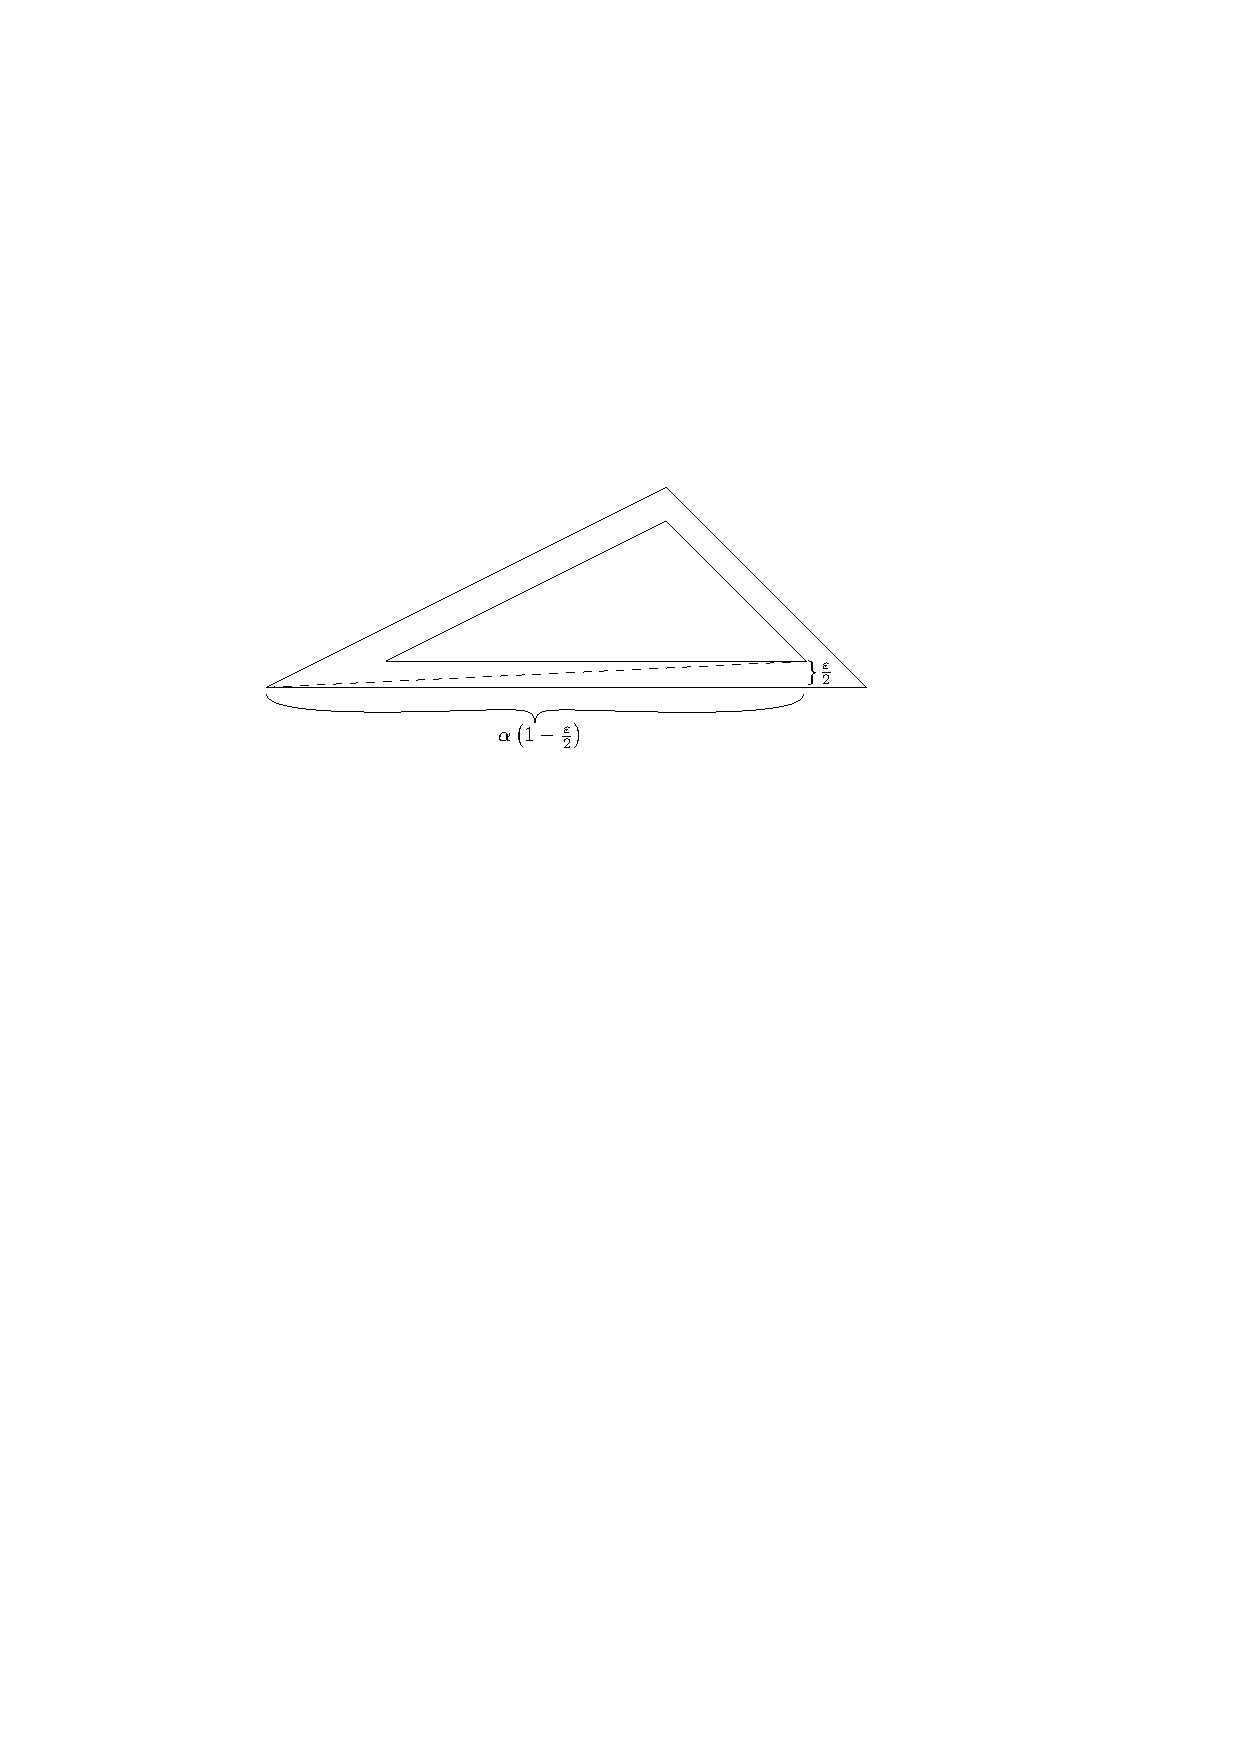
\includegraphics[width=0.6\linewidth]{figs/triangle_shadow}
    \figlab{triangle_with_shadow}
\end{figure}


\bibliographystyle{alpha} 
%\bibliography{shortcuts,geometry}
\bibliography{ft_spanner}

\end{document}
